\documentclass[diplomskirad]{fer}
% Dodaj opciju upload za generiranje konačne verzije koja se učitava na FERWeb
% Add the option upload to generate the final version which is uploaded to FERWeb


%--- PODACI O RADU / THESIS INFORMATION ----------------------------------------

% Naslov na engleskom jeziku / Title in English
\title{A system for recognizing voice commands in real-time on edge devices}

% Naslov na hrvatskom jeziku / Title in Croatian
\naslov{Sustav za prepoznavanje govornih naredbi u stvarnom vremenu na rubnim uređajima}

% Broj rada / Thesis number
\brojrada{720}

% Autor / Author
\author{Luka Balić}

% Mentor 
\mentor{Prof. Hrvoje Džapo}

% Datum rada na engleskom jeziku / Date in English
\date{February 14th, 2025}

% Datum rada na hrvatskom jeziku / Date in Croatian
\datum{14. veljače 2025.}

%-------------------------------------------------------------------------------


\begin{document}


% Naslovnica se automatski generira / Titlepage is automatically generated
\maketitle


%--- ZADATAK / THESIS ASSIGNMENT -----------------------------------------------

% Zadatak se ubacuje iz vanjske datoteke / Thesis assignment is included from external file
% Upiši ime PDF datoteke preuzete s FERWeb-a / Enter the filename of the PDF downloaded from FERWeb
\zadatak{zadatak.pdf}


%--- ZAHVALE / ACKNOWLEDGMENT --------------------------------------------------

\begin{zahvale}
  % Ovdje upišite zahvale / Write in the acknowledgment
  Hvala svima...
\end{zahvale}


% Odovud započinje numeriranje stranica / Page numbering starts from here
\mainmatter


% Sadržaj se automatski generira / Table of contents is automatically generated
\tableofcontents

%\cite{1}
%\chapter{primjer}
\label{pog:primjer}

Neki od radova koje ćemo citirati su \cite{6248073,6247753,ghiglia_pritt_phase_unwrapping,hartley2003multiple,4250461,123DCatch}.
Trebaju nam samo radi testiranja kako izgleda referenciranje rada s konferencije, rada iz časopisa, knjige i Internetske stranice.

\begin{figure}[htb]
  \centering
  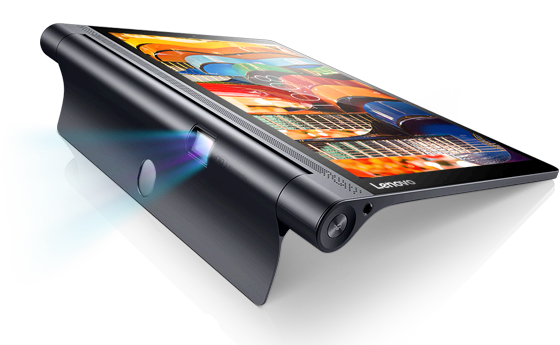
\includegraphics[width=0.38\linewidth]{Figures/lenovo_yoga_tab3_pro_front.png} 
  \caption{Moja prva slika}
  \label{slk:prvaslika}
\end{figure}

Referenciramo se na sliku \ref{slk:prvaslika} u sredini rečenice, zatim prije zareza \ref{slk:prvaslika}, te zatim na kraju rečenice \ref{slk:prvaslika}.
Upravo smo testirali radi li naredba \verb|\ref| ispravno u slučaju kada nakon nje slijedi točka.

Sada slijedi jedna jednadžba:
\begin{equation}
  \label{jed:prvajednadzba}
  \int_{-\infty}^{+\infty}f(t)\,dt=F(\omega)
\end{equation}
Jednadžba \eqref{jed:prvajednadzba} je moja prva jednadžba koja defnira par $f(t)\ufrek F(\omega)$ ili $F(\omega)\uvrem f(t)$.

\chapter{Uvod}
\label{pog:uvod}

%\section{Tiny ML}

Modeli strojnog učenja revolucionarizirali su tehnologiju koju koristimo u svakodnevnom
životu tako što su omogućili računalima učenje iz podataka kojima raspolažu u svrhu
donošenja odluka u situacijama za koje nisu eksplicitno programirana. Tradicionalno
su takvi modeli bili namijenjeni za računala visokih performansi i neograničavajućih
resursa, međutim sve bržim razvojem IoT (engl. \textit{Internet of Things}) područja te
zahvaljujući pristupačnoj cijeni mikrokontrolerskih sustava, počela je prilagodba
modela strojnog učenja za takve sustave. Na prvi pogled dva nespojiva svijeta
su se susrela te pronašla svoju primjenu u raznovrsnim sustavima.
Tiny ML (engl. \textit{Tiny Machine Learning}) je naziv koji se odnosi na implementaciju
modela strojnog učenja na uređaje ograničenih resursa kao što su mobilni telefoni
i mikrokontroleri. Glavne karakteristike modela namijenjenih za takve sustave su
relativno malen memorijski otisak, mogućnost odziva u stvarnom vremenu,
smanjenje potrošnje i internetskog prometa te sigurnost \cite{tinyml}. Sustav
implementiran kroz ovaj rad ima zadatak prepoznati unaprijed zadane glasovne
naredbe te pokrenuti izvršavanje određenog posla vezanog uz specifičnu naredbu.

%\section{Opis problema}

Okruženi smo digitalnim glasovnim asistentima kao što su Googleov Assistant,
Appleova Siri te Amazonova Alexa. Ovakvi sustavi mogu u vrlo kratkom
roku pružiti zatražene informacije i bez ikakvog problema komunicirati s osobom
koja ih koristi. Za prepoznavanje i obradu ljudskog govora i dohvaćanje bitnih
informacija zaduženi su modeli kojima je potrebna velika procesorska moć i dovoljno
prostora za pohranu te se zbog toga taj dio posla odrađuje na serverskim računalima.
Takav sustav podrazumijeva konstantnu internetsku vezu uz stabilan i dugotrajan
izvor električne energije. Kada bi mobilni uređaji slali konstantan tok zvučnih podataka
na server, brzo bi ispraznili bateriju te nepotrebno koristili mobilne podatke za
pristup internetu. Zbog toga su takvi sustavi osmišljeni da čekaju naredbu za
početak komunikacije, a tek onda uspostave vezu sa serverom. Međutim, i dalje
nam ostaje problem konstantne akvizicije ulaznih zvučnih podataka te prepoznavanje
naredbe kao što je ”Hey Google” ili nešto slično. U ovoj situaciji savršenu primjenu
pronašli su procesori izrazito male potrošnje na kojima je moguće implementirati
optimizirane modele strojnog učenja. Takav procesor bi konstantno akvizirao podatke
s mikrofona te lokalno, uz pomoć treniranog modela, čekao ključnu riječ nakon
koje bi dao znak cijelom sustavu da se može ”probuditi” iz stanja niske
potrošnje te odraditi svoj posao. Ovakvim pristupom postignuta je efikasnost, niska
potrošnja, brz odaziv, smanjena je potrošnja internetskih podataka te možda i
najvažnija stvar - privatnost. Naime, nema potrebe za konstantnim slanjem glasovnih
podataka na server što omogućuje da na server dospiju samo glasovni isječci u
trenucima u kojima želimo.

\chapter{Struktura sustava}
\label{pog:struktura_sustava}
\chapter{Neuronska mreža}
\label{pog:neuronska_mreza}

\section{Općenito}

Okosnica cjelokupnog sustava za prepoznavanje izgovorenih naredbi je neuronska mreža.
Neuronska mreža ili preciznije umjetna neuronska mreža je računalni model inspiriran
biološkom strukturom neurona u mozgu čovjeka. Predstavlja jedan od najkorištenijih modela 
u dubokom učenju. Sastoji se od čvorova (neurona) i jednosmjernih
veza između njih (sinapsa) koji na taj način tvore usmjereni graf. Čvorovi su grupirani u slojeve,
a svaki od njih je povezan s čvorovima iz susjednog sloja na određeni način. Način na koji su
određeni slojevi međusobno povezani određuje vrstu sloja. 

Jednostavan primjer strukture neuronske mreže je potpuno povezani sloj (engl. fully connected layer
ili dense layer) koji se često koristi kao osnovni građevni blok u umjetnim neuronskim mrežama \cite{dense}.
U potpuno povezanom sloju svaki čvor jednog sloja povezan je sa svakim čvorom susjednog sloja.
Ovakva struktura omogućava mreži fleksibilno učenje složenih odnosa između ulaznih i izlaznih podataka.

\begin{figure}[htb]
  \centering
  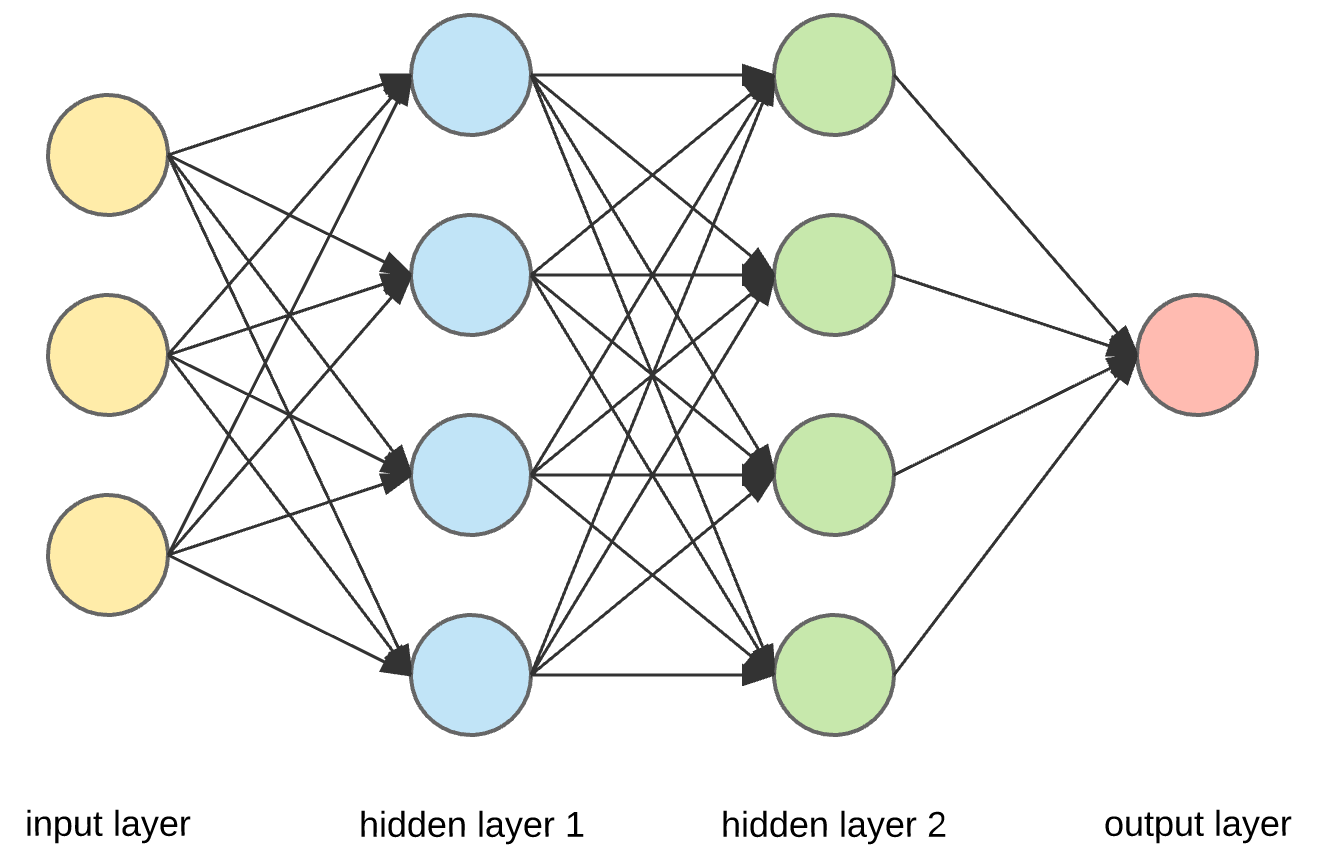
\includegraphics[width=0.5\linewidth]{Chapters/neuronska_mreza/dense_layer.png} 
  \caption{Potpuno povezani slojevi \cite{dense}}
  \label{pic:dense_layer}
\end{figure}

Na slici \ref{pic:dense_layer} prikazana je struktura neuronske mreže koja se sastoji od ulaznog sloja,
dva potpuno povezana sloja te izlaznog sloja. Srednji slojevi (svi osim ulaznog i izlaznog)
se još nazivaju i skriveni slojevi jer kad koristimo model neuronske mreže, gledamo
na njega kao na crnu kutiju koja na ulazu prima vrijednosti te na izlazu daje vrijednosti
izračunate kroz sve skrivene slojeve \cite{fully_connected}.

Svaka veza između pojedinih čvorova ima određenu vrijednost koju nazivamo težina, a svaki čvor
zapravo predstavlja funkciju koja može aktivirati svoj izlaz i vezu sa sljedećim čvorom.

\begin{equation}
  \label{eq:neuron_activation}
  a = f\left(\sum_{i=1}^n w_i x_i + b\right)
\end{equation}

Jednadžba \eqref{eq:neuron_activation} modelira ponašanje pojedinog čvora u mreži. Aktivacijska
funkcija \( f \) je vrlo bitna u odvajanju bitnih od nebitnih utjecaja pojedinih čvorova na sljedeći
čvor. Također, ona nam omogućava modeliranje složenijih nelinearnih odnosa \cite{activation_fcn}.
Kada bi čvor bio modeliran
bez aktivacijske funkcije svako preslikavanje koje bi činio bi bilo linearno, a zbog toga što nam
svaka kompozicija linernih funkcija daje opet linearnu funkciju, cjelokupna mreža ne bi bila sposobna
modelirati kompleksnije stvari. Sastavnice modela čvora su sljedeće:

\begin{itemize}
  \item \( a \): izlazna vrijednost čvora (aktivacija)
  \item \( f \): aktivacijska funkcija
  \item \( w_i \): težina i-tog ulaznog čvora (čvor u prijašnjem sloju)
  \item \( x_i \): vrijednost i-tog ulaznog čvora (njegova aktivacija)
  \item \( b \): pomak
  \item \( n \): broj čvorova u prijašnjem sloju koji imaju vezu s modeliranim čvorom
\end{itemize}

Povezivanjem više ovako definiranih čvorova gradimo neuronske mreže. Ulaz u neuronsku mrežu 
je informacija na temelju koje će na izlazu iz mreže biti vrijednost izračunata pomoću svih
slojeva u mreži. Kako bi vrijednosti na izlazu iz mreže imale smisla, tj. davale korisnu
informaciju, potrebno je trenirati mrežu. Treniranje mreže, u općem slučaju nadziranog strojnog
učenja, podrazumijeva korištenje označenog skupa podataka koji je istog oblika kao i podaci
koji će biti na ulazu u mrežu tijekom korištenja same mreže. Arhitektura mreže (vrsta, veličina
i broj slojeva) određena je prije samog treniranja, dok se težine, pomaci te samim time i 
razine aktivacija uče, tj. treniraju. Treniranje je proces u kojem se neuronska mreža "hrani" 
označenim skupom podataka (označeni skup prestavlja podatke za koje znamo što bi mreža trebala
dati na izlazu) te provjerava koliko izlazi odstupaju od prave oznake. Na početku su sve težine
uglavnom inicijalizirane na nulu. Podatak se predaje ulaznom sloju, prolazi kroz sve skrivene
slojeve te na izlazu mreža izbaci određenu vrijednost koja se s očekivanom uspoređuje pomoću
funckije gubitka. Takva funkcija predstavlja koliko izlazi iz mreže odstupaju od očekivanih.

%Na slici \ref{pic:feedforward} prikazana je jednostavna neuronska mreža čiji izlaz daje određenu
%vrijednost funkciji gubitka.
%\begin{figure}[htb]
%  \centering
%  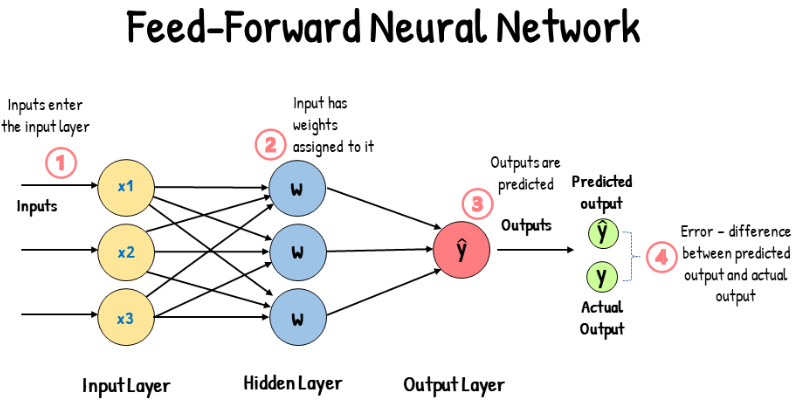
\includegraphics[width=0.5\linewidth]{Chapters/neuronska_mreza/feed_forward.png} 
%  \caption{Dense}
%  \label{pic:feedforward}
%\end{figure}


Cilj svakog treniranja jest smanjiti vrijednost funkcije gubitka. Stoga se sve težine u mreži
ažuriraju na način da njihove promjene pomaknu trenutno stanje mreže u smjeru negativne derivacije
funckije gubitka (gradijentni spust). Takvim pristupom, mreža kroz iteracije s novim podacima smanjuje funkciju gubitka
(efektivno daje sve točnije predikcije). Težine se ažuriraju od izlaznog sloja prema ulaznom 
(eng. backpropagation) jer na izlaz pojedinog sloja utječu njegovi ulazi, tj. izlazi prijašnjeg
sloja (izlaz svakog sloja je funkcija izlaza prijašenjeg sloja, a kad izračunamo derivaciju
funkcije, pomjenom njenih ulaza znamo u kojem smjeru će se mijenjati vrijednost same funkcije).


%Na slici \ref{pic:backprop} prikazana je mreža i način ažuriranja težina "unazad".
%\begin{figure}[htb]
%  \centering
%  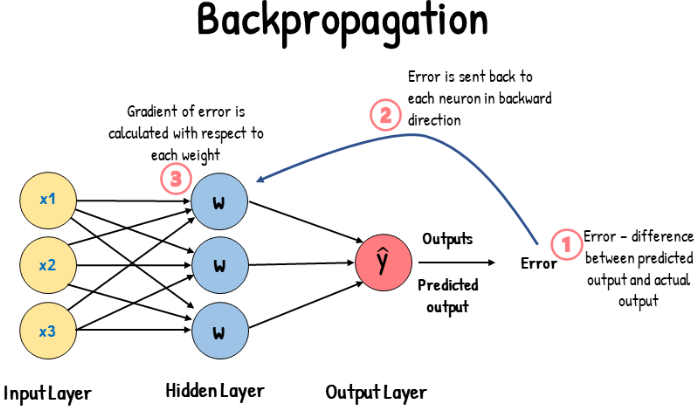
\includegraphics[width=0.5\linewidth]{Chapters/neuronska_mreza/backprop.png} 
%  \caption{Dense}
%  \label{pic:backprop}
%\end{figure}

Bez smanjenja općenitosti, funkcija gubitka prikazana je na trodimenzionalnom grafu
na slici \ref{pic:descent}. Složene arhitekture mreža će imati više dimenzija zbog većeg broja
težina \( w_i \). Cilj svakog treniranja mreže je doći što bliže minimumu ovakve funckije.
Svakom iteracijom pomičemo se sve bliže minimumu, taakva vrsta optimizacije naziva se
gradijentni spust.

\begin{figure}[htb]
  \centering
  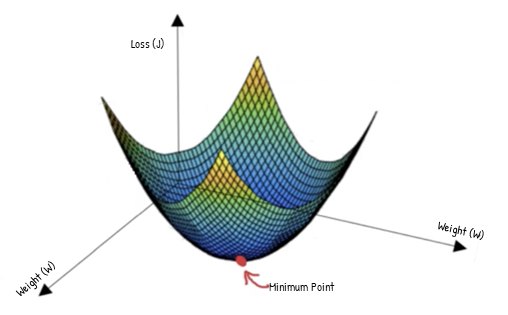
\includegraphics[width=0.5\linewidth]{Chapters/neuronska_mreza/descent.png} 
  \caption{Funkcija gubitka \cite{desc}}
  \label{pic:descent}
\end{figure}


%ostala poglavlja
\section{Konvolucijska neuronska mreža}
\label{sec:cnn}

Konvolucijska neuronska mreža (engl. \textit{Convolutional neural network ili CNN}) je vrsta 
umjetne neuronske mreže koja je pogodna je za obradu podataka s rešetkastom (matričnom)
topologijom, a najviše se koristi za rješavanje problema iz područja klasifikacije slika
te računalnog vida. Inspirirane su načinom funkcioniranja moždanog korteksa 
zaduženog za vid kod sisavaca \cite{pycodemates}. Obrada slike koju vide sisavci
funkcionira hijerarhijski, tj. u mozgu se ne obrađuje cjelokupna slika odjednom,
nego postoje jednostavnije stanice koje su zadužene za prepoznavanje osnovnijih
oblika koji se nakon toga stapaju u složenije. Naposljetku 
organizam može prepoznati cjelokupnu sliku koju gleda očima.
Veza između prepoznavanja slika i problema klasifikacije glasovnih naredbi možda nije
vidljiva na prvu. Međutim, generirana matrica značajki iz poglavlja \ref{sec:gen} predstavlja
upravo dvodimenzionalnu
sliku koja se može koristiti kao ulaz u konvolucijsku neuronsku mrežu.

Računalni modeli koji koriste strukturu sličnu opisanoj mogu iz
podataka koji su u takvom obliku izvući značajke samostalno što znači da nema
potrebe za korištenjem metoda koje eksplicitno izvlače bitne značajke iz matričnih podataka
\cite{1}. Arhitektura najjednostavnije konvolucijske neuronske mreže
uključuje:

\begin{itemize}
    \item \textbf{Ulaz}: ulazni sloj modela, prima matrični podatak
    \item \textbf{Konvolucijski sloj}: osnovni sloj modela. Njegov glavni zadatak
          je ekstrakcija značajki iz ulaznih podataka. Vidi \ref{sub:conv}.
    \item \textbf{Sloj za poduzorkovanje}: smanjuje dimenzionalnost (vidi \ref{sub:pooling})
    \item \textbf{Sloj za poravnavanje}: spaja konvolucijski i potpuno povezani dio (vidi \ref{sub:flat})
    \item \textbf{Potpuno povezani sloj}: povezuje značajke s klasifikacijom (vidi \ref{sub:dense})
    \item \textbf{Izlaz}: izlazni sloj, daje vjerojatnosti klasifikacije (vidi \ref{sub:output})
\end{itemize}

\begin{figure}[htb]
    \centering
    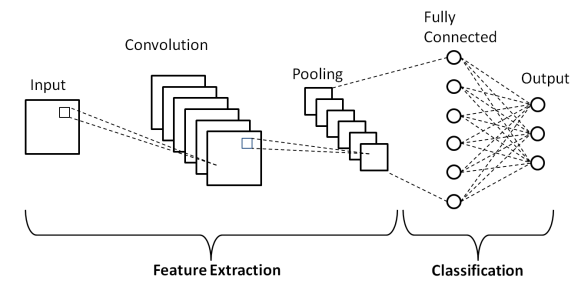
\includegraphics[width=0.5\linewidth]{Chapters/neuronska_mreza/CNN/cnn.png} 
    \caption{Jednostavna CNN \cite{1}}
    \label{pic:cnn}
\end{figure}

Na slici \ref{pic:cnn} prikazana je opisana struktura. Prva tri sloja grupirana su
u dio koji služi za ekstrakciju značajki iz ulaznih podataka, a posljednja dva
sloja služe za klasifikaciju. Složenije arhitekture mreže mogu imati veći broj
konvolucijskih slojeva (nakon svakog se nalazi sloj za poduzorkovanje) te veći broj
složenijih ili manje složenih potpuno povezanih slojeva.

\subsection{Konvolucijski sloj}
\label{sub:conv}

Najbitniji dio ovakvog tipa neuronske mreže je konvolucijski sloj 
(engl. \textit{convolutional layer}) zbog toga što se
u njemu događa konvolucija. Konvolucija (u neuronskim mrežama) je proces kojim se
iz ulazne matrice podataka (slike) na izlazu dobije matrica značajki ili
mapa značajki. Neka je ulazna matrica oblika \( x \in M_{mn}(\mathbb{R}) \).
Umjesto težina (kao kod potpuno povezanog sloja), konvolucijski sloj koristi
matricu \( \omega \in M_{pr}(\mathbb{R}) \) koju nazivamo filtar ili
jezgra (engl. \textit{kernel}) \cite{keras_layers}. Svaki konvolucijski 
sloj može imati proizvoljan broj filtara. Izlazna (u ovom slučaju dvodimenzionalna)
mapa značajki tada se računa na sljedeći način:

\begin{equation}
h = \omega * x,
\end{equation}

pri čemu \( * \) označava operaciju konvolucije te vrijedi:

\begin{equation}
h(i, j) = (\omega * x)(i, j) = 
\sum_{k=0}^{p-1} \sum_{l=0}^{r-1} x(i + k, j + l) \omega(k, l).
\end{equation}

Formula koja se zapravo koristi naziva se unakrsna korelacija, međutim, zbog sličnosti s 
formulom konvolucije, mreža nosi takav naziv \cite{gracan2020}. Na slici 
\ref{pic:convolution} prikazan je proces koji se događa tijekom prolaska 
ulaznog podatka kroz konvolucijski sloj. Ulaz (engl. \textit{input}) se konvolucijski množi
s jezgrom kako bi se dobila izlazna matrica značajki \cite{cnn_how}. U slučaju prikazanom na slici,
ulazna slika je veličine \(4 \times 4\), dok je jezgra veličine \(3 \times 3\). Prvo se podmatrica ulaznog
podatka veličine jednake veličini jezgre (\(3 \times 3\)) skalarno množi s jezgrom. Izlaz je 
skalarni umnožak na koji se može dodati konstantna vrijednost (engl. \textit{bias}). Nakon
toga se jezgra pomiče po ulaznoj matrici, tj. sljedeći element izlazne matrice je
skalarni umnožak jezgre i sljedeće podmatrice ulaznog podatka. Koliko će se jezgra
pomaknuti određuje pomak (engl. \textit{stride}). U slučaju na slici \ref{pic:convolution}
pomak iznosi jedan.

\begin{figure}[htb]
      \centering
      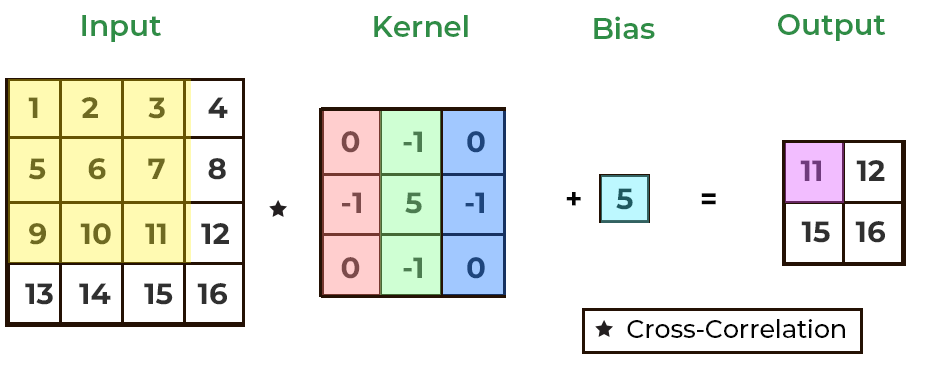
\includegraphics[width=0.5\linewidth]{Chapters/neuronska_mreza/CNN/convolution.png} 
      \caption{Konvolucija \cite{convolution}}
      \label{pic:convolution}
\end{figure}

Rezultat opisanog procesa je mapa značajki koja je manja od ulazne, a njena veličina
obrnuto proporcionalno ovisi o veličini jezgre te pomaku \cite{cnn_whatis}. 

Slično procesu koji se odvija u mozgu čovjeka, opisana struktura omogućava hijerarhijsko učenje.
Naime, svaki konvolucijski sloj sadrži jezgre koje su zadužene za lokalno pretraživanje
određenih uzoraka. Upravo konvolucijom izvlačimo stvari koje su slične između različitih
ulaznih slika. Koje jezgre se trebaju koristiti određuje proces učenja (treniranja
mreže) koji prepoznaje lokalne sličnosti između različitih primjera. Ako se mreža sastoji
od više uzastopnih konvolucijskih slojeva, prvo će naučiti najjednostavnije
oblike, a zatim u sljedećem sloju takvim oblicima slagati složenije uzorke. Također,
još jedna prednost konvolucijskog sloja je u dijeljenju parametara. Takav sloj nema vezu 
svakog neurona sa svakim ulaznim, nego se težine dijele unutar određene jezgre. Zapravo se
cijeli proces učenja svodi na nalaženje odgovarajućih jezgri koje će prepoznati uzorke \cite{pycodemates}.
U slučaju dvodimenzionalne ulazne slike, broj parametara ovakvog sloja iznosit će:

\begin{equation}
    N = (n \cdot m \cdot C_{\text{in}} + 1) \cdot C_{\text{out}}
\end{equation}

gdje su:
\begin{itemize}
    \item \(N\): ukupni broj parametara,
    \item \(n\) i \(m\): visina i širina filtra (jezgre),
    \item \(C_{\text{in}}\): broj ulaznih kanala (npr. 1 za crno-bijele slike, 3 za RGB slike),
    \item \(+1\): konstanta svakog filtra,
    \item \(C_{\text{out}}\): broj filtara (odnosno mapa izlaznih značajki).
\end{itemize}

Kako bi se bolje dočarala razlika u broju parametara između ovakvog sloja i potpuno povezanog sloja,
kao primjer može se uzeti slika \ref{pic:convolution}. Ulazna slika je veličine \(4 \times 4\),
jezgra \(3 \times 3\), a izlaz 
\(2 \times 2\). Neka je slika jednokanalna, a broj jezgri jedan (sve kao na slici). Konvolucijski sloj
će u tom slučaju imati 10 parametara, dok će potpuno povezani sloj (16 ulaznih vrijednosti, 4 izlazne te
4 konstante za svaki neuron) imati 68 parametara! Formula za broj parametara u tom slučaju
je sljedeća:

\begin{equation}
    N = n_{\text{in}} \cdot n_{\text{out}} + n_{\text{out}}
\end{equation}

gdje su:
\begin{itemize}
    \item \(N\): ukupni broj parametara,
    \item \(n_{\text{in}}\): broj ulaznih neurona,
    \item \(n_{\text{out}}\): broj izlaznih neurona.
\end{itemize}

Također, kao što je opisano u poglavlju \ref{pog:neuronska_mreza} vrijednost neurona (čvora) na
izlazu iz sloja potrebno je provući kroz aktivacijsku funkciju. Postoje različite vrste funkcija
koje se koriste u različitim granama strojnog i dubokog učenja \cite{activation_fcn}, a za
primjenu u konvolucijskim slojevima, najefektivnija se pokazala ReLu (engl. \textit{Rectified linear units})
\cite{relu}. To je funkcija koja vraća nulu ako joj je ulaz negativan, a za svaki pozitivan
ulaz samo prosljeđuje istu vrijednost na izlaz. Modelirana je formulama \ref{eq:relu1} i 
\ref{eq:relu2}, a prikazana je na slici \ref{pic:relu}. 

\begin{equation}
    f(x) = \max(0, x)
    \label{eq:relu1}
\end{equation}

\begin{equation}
    f(x) = 
    \begin{cases} 
        0, & \text{ako } x < 0, \\
        x, & \text{ako } x \geq 0.
    \end{cases}
    \label{eq:relu2}
\end{equation}

\begin{figure}[htb]
    \centering
    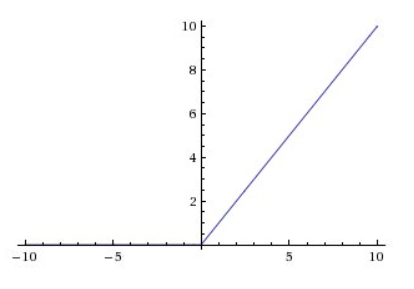
\includegraphics[width=0.5\linewidth]{Chapters/neuronska_mreza/CNN/relu.png} 
    \caption{ReLu \cite{relu}}
    \label{pic:relu}
\end{figure}

Prednosti ReLu funkcije nad drugim aktivacijskim funkcijama je u tome što za negativne
ulaze uopće ne aktivira neuron što izuzetno povećava efikasnost. Druga prednost je u tome
što izlaz linearno raste s porastom ulazne vrijednosti što znači da nikad neće ući
u zasićenje. Ta osobina je važna jer utječe na izgled funkcije gubitka te ubrzava
konvergenciju gradijentnog spusta prema minimumu funkcije gubitka \cite{activation_fcn}.


\subsection{Sloj za poduzorkovanje}
\label{sub:pooling}
Sloj za poduzorkovanje (engl. \textit{pooling layer}) služi smanjenju dimenzionalnosti matrice
značajki na izlazu iz konvolucijskog sloja. Najčešće korištene tehnike su maksimalno 
(engl. \textit{max pooling}) i prosječno poduzorkovanje (engl. \textit{average pooling}). 
Radi tako da više 
susjednih vrijednosti spoji u jednu te tako na svom izlazu da matricu manjih dimenzija 
\cite{pooling1}. Na taj način postupno smanjuje broj parametara, smanjuje broj
operacija potrebnih za daljnje računanje te ono najbitnije, kontrolira
prenaučenost \cite{cnn_whatis}. Na slici \ref{pic:pooling} prikazane su obje navedene vrste poduzorkovanja.

\begin{figure}[htb]
    \centering
    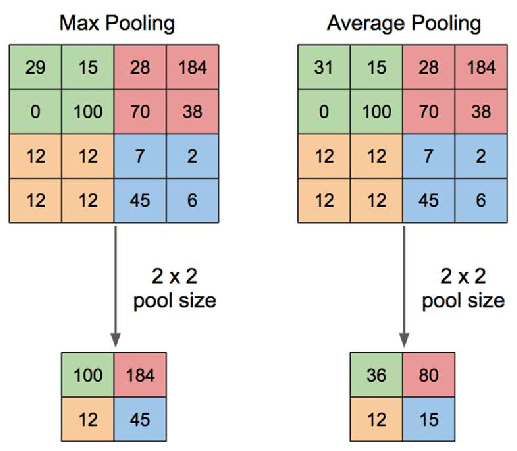
\includegraphics[width=0.5\linewidth]{Chapters/neuronska_mreza/CNN/pooling.png} 
    \caption{Poduzorkovanje \cite{pooling1}}
    \label{pic:pooling}
\end{figure}

Prosječno poduzorkovanje izglađuje sliku (engl. \textit{smoothing}). Zbog toga oštri detalji slike
mogu biti izgubljeni što znači da se određene značajke možda neće prepoznati kada se 
koristi ova metoda. Maksimalno uzorkovanje odabire piksele s najvećom vrijednošću iz slike,
a oni su se pokazali kao najbitnije značajke jer daju najbolje rezultate \cite{cnn_whatis}.
Suprotno tome, minimalno uzorkovanje (engl. \textit{min pooling}) odabralo bi piksele s najmanjom
vrijednošću, međutim ono se najrjeđe koristi.

\subsection{Sloj za poravnavanje}
\label{sub:flat}
Sloj za poravnavanje (engl. \textit{flatten layer}) je sloj koji dolazi nakon posljednjeg sloja
za poduzorkovanje. Njegova jedina zadaća je poravnati izlaz iz prijašnjeg sloja.
Ovaj sloj ništa ne računa, ništa ne uči, jedina zadaća mu je od ulaznih mapa značajki
napraviti jedan vektor koji je onda moguće povezati na potpuno povezani sloj. Zbog
toga se često izostavi iz skica koje prikazuju strukture CNN-ova kao što je slučaj
na slici \ref{pic:cnn}. Na slici \ref{pic:flatten} prikazana je uloga ovog sloja.

\begin{figure}[htb]
    \centering
    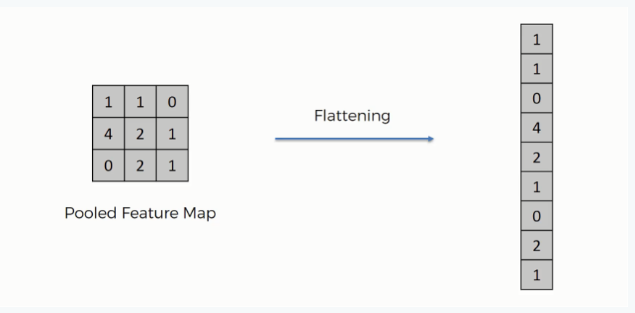
\includegraphics[width=0.5\linewidth]{Chapters/neuronska_mreza/CNN/flatten.png} 
    \caption{Sloj za poravnjavanje \cite{flatten}}
    \label{pic:flatten}
\end{figure}


\subsection{Potpuno povezani sloj}
\label{sub:dense}
Potpuno povezani sloj (engl. \textit{fully connected layer}) detaljnije je pojašnjen u poglavlju
\ref{pog:neuronska_mreza}. Nakon prijašnjih slojeva koji su služili za izvlačenje
značajki iz ulaznih podataka, na red dolazi klasifikacija. Budući da je prethodnik
prvom ovakvom sloju sloj za poravnavanje, ne postoji problem sa spajanjem ovog sloja na dosad
objašnjenu strukturu. Uloga ovog sloja (ili više ovakvih slojeva) je, najjednostavnije
rečeno, klasifikacija. Značajke naučene tijekom konvolucije se ovdje predaju gustoj mreži
neurona koja je sposobna odraditi posao do kraja, tj. naučiti kako različite značajke
pridonose određenoj izlaznoj klasi.

\subsection{Izlazni sloj}
\label{sub:output}
Izlazni (engl. \textit{output layer}) je posljednji sloj potpuno povezanog sloja, a time ujedno i cijele
neuronske mreže. Ima onoliko neurona koliko se želi imati klasa, a pojedina vrijednost
neurona predstavlja vjerojatnost pripadnosti određenoj klasi. Da bi to stvarno funkcioniralo na takav
način, potrebno je odrediti prikladnu aktivacijsku funkciju. Funkcija koja to radi 
naziva se funkcija \textit{softmax}. 
Formalno, \( \text{softmax} : \mathbb{R}^n \to \mathbb{R}^n \),
gdje je \( k \)-ta komponenta izlaznog vektora definirana kao:
\begin{equation}
\text{softmax}_k(x_1, \dots, x_n) = \frac{\exp(x_k)}{\sum_{j} \exp(x_j)}
\end{equation}

Funkcija softmax radi dvije ključne stvari:
\begin{itemize}
    \item Normalizira sve vrijednosti tako da njihov zbroj bude \( 1 \), tj. izlazni vektor 
        predstavlja distribuciju vjerojatnosti.
    \item Pojačava veće vrijednosti (čini ih dominantnijima) i smanjuje manje vrijednosti.
\end{itemize}

Funkcija nosi naziv \textit{softmax} jer odgovara funkciji \( \max \), ali je "meka" u smislu
da je neprekidna i diferencijabilna, za razliku od klasične \( \max \) funkcije 
\cite{snajder2023logreg}.

\begin{figure}[htb]
    \centering
    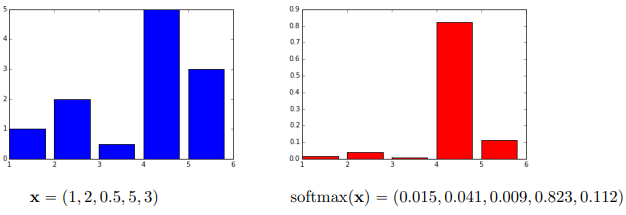
\includegraphics[width=0.6\linewidth]{Chapters/neuronska_mreza/CNN/softmax.png} 
    \caption{Softmax \cite{snajder2023logreg}}
    \label{pic:softmax}
\end{figure}

\subsection{Regularizacija odbacivanjem težina}
Regularizacija je postupak kojim se smanjuje složenost modela kako bi se spriječila
prenaučenost (engl. \textit{overfitting}). Prenaučenost se događa kada model ima preveliku  
sposobnost prilagodbe podacima za treniranje, ali ne i za podacima za testiranje.
U neuronskim mrežama je, uz sloj za poduzorkovanje, implementirana u obliku sloja koji tijekom
treniranja slučajnim odabirom postavlja određeni postotak 
težina u modelu na nulu (engl. \textit{dropout layer}).

\subsection{Poznate arhitekture konvolucijskih mreža}
Arhitektura konvolucijske mreže je ključni faktor koji određuje njene performanse i
učinkovitost. Broj konvolucijskih slojeva, izgled istih (broj filtara, njihova veličina,
pomak), vrsta slojeva za poduzorkovanje te broj i veličina potpuno povezanih slojeva znatno
utječu na brzinu izvođenja i preciznost klasifikacije. Naravno, ne postoji jedan recept koji
najbolje radi na svim vrstama ulaznih podataka, nego različite arhitekture daju bolje rezultate
u određenim situacijama. Dobro je istaknuti određene arhitekture koje imaju povijesno značenje 
zbog toga kako su utjecale na područje istraživanja u dubokom učenju\cite{indian}:

\begin{itemize}
    \item \textbf{LeNet-5 (1998):} 
    CNN sa 7 slojeva dizajnirana za klasifikaciju rukom pisanih brojeva na slikama 
    veličine \(32 \times 32\) piksela u sivim tonovima. Koristila se u bankama za čitanje čekova 
    i bila je prvi značajan korak u korištenju CNN-a u stvarnom svijetu.

    \item \textbf{AlexNet (2012):} 
    Proširena verzija LeNet-a s dubljom arhitekturom (5 konvolucijskih i 3 potpuno povezana 
    sloja). Prva mreža koja je koristila ReLU aktivaciju za brže treniranje. Značajno smanjila
    stopu pogreške na ILSVRC natjecanju i popularizirala duboko učenje.

    \item \textbf{GoogleNet (Inception V1) (2014):} 
    22-slojna mreža s inovativnim \emph{inception module}, koji koristi male konvolucije za 
    smanjenje broja parametara (sa 60 milijuna na samo 4 milijuna). Pobjednik ILSVRC 2014 s 
    top-5 pogreškom manjom od 7\%. Performanse su usporedive s ljudskim prepoznavanjem slika.

    \item \textbf{VGGNet (2014):} 
    Mreža sa 16 konvolucijskih slojeva koja koristi samo \(3 \times 3\) konvolucije s povećanim
    brojem filtara. Iako je jednostavna u dizajnu, ima 138 milijuna parametara, što je čini 
    računalno zahtjevnom za treniranje i implementaciju.
\end{itemize}
\section{Skup podataka za treniranje}
\label{sec:dataset}

Prvi korak u izgradnji sustava koji koristi bilo kakav tip modela strojnog učenja
je odabir i priprema prikladnog skupa podataka na kojem će se taj model trenirati.
Budući da je cilj sustava prepoznavanje govornih naredbi (engl. \textit{keyword spotting}),
prikladan otvoreni skup podataka za tu svrhu je skup za treniranje prepoznavanja ograničenog
skupa govornih naredbi \cite{speechcommandsv2}. Riječ je o skupu koji
se sastoji od oko 105000 zvučnih isječaka duljine oko jedne sekunde (frekvencija
zapisa je 16 kHz) u kojima ljudi
izgovaraju jednu od 35 različitih riječi. Također, skup ima nekoliko vrsta 
pozadinske buke koja je ključna za rad ovakvog sustava u stvarnim uvjetima. 
U prikupljanju podataka sudjelovalo je oko 2600 ljudi iz cijelog svijeta.
U privitku je prikazana tablica koja prikazuje od kojih se riječi skup sastoji
te koliko snimaka pojedinih riječi postoji \ref{tab:word_frequency}.


\section{Priprema podataka}
\label{sec:data}

Nakon odabira skupa na kojem će model biti treniran, potrebno je pripremiti
podatke. Zbog ograničenih resursa na mikrokontrolerskom sustavu, nije moguće
(a niti potrebno za konkretnu namjenu) izgraditi sustav koji će moći
prepoznati sve riječi iz skupa. Potrebno je odabrati samo podskup
naredbi koje će sustav uspješno klasificirati. Cjelokupni
proces pripreme podataka, treniranja i validacije modela popraćen je
Jupyter bilježnicom koja se nalazi u GitHub repozitoriju
\cite{balic_keyword_spotting}.

Projektirani sustav mora moći prepoznati naredbe koje su izgovorene.
Zbog toga, mora biti sposoban odbaciti sve ono što nije naredba koja se
nalazi u odabranom skupu. Budući da će sustav treba raditi u stvarnim uvjetima,
jedna od kategorija (klasa)
na kojoj model mora biti treniran je i pozadinska buka. Ona je sveprisutna te 
zbog toga sustav treba biti otporan takav tip zvukova. Odabrani skup podataka
sadrži zvučne zapise kao što je zvuk perilice posuđa, zvuk vode koja teče
iz slavine, bijeli šum te ružičasti šum. Bijeli šum je vrsta
signala koji u sebi sadrži sve frekvencije i sve imaju isti intenzitet,
dok se ružičasti šum također sastoji od svih frekvencija, ali veći intenzitet
imaju niže frekvencijske komponente \cite{noise}. Takvi zvukovi dobro predstavljaju
tipičnu okolinu u kojoj bi se sustav mogao nalaziti. Međutim, zbog toga što skup
podataka sadrži
svega nekoliko minuta takvih zvučnih zapisa, potrebno je na neki način dopuniti
taj podskup podataka. Naime, mreža koju treniramo će preferirati neku od klasa
ako takvih primjera ima mnogo više od primjera ostalih klasa. Drugim riječima,
skup podataka za treniranje mora biti balansiran tj. primjera iz svake klase treba
biti otprilike jednak broj \cite{balance}. Uz to, za rad u stvarnom svijetu, nije 
loše u skup
dodati zvučni zapis snimljen upravo na sustavu koji će i akvizirati podatke iz okoline.
Budući da su svi zvučni zapisi 
riječi u skupu podataka duljine od otprilike jedne sekunde, pozadinske zvukove
je potrebno skratiti na identičnu duljinu kako bi mreža mogla primati vrlo 
precizno definiranu vrstu ulaznih podataka. O broju riječi iz klasa koje su odabrane 
kao naredbe ovisit će koliko je potrebno isječaka koji će predstavljati
klasu pozadinskih zvukova. Metoda kojom se lako može umnožiti broj pozadinskih 
zvukova zove se augmentacija.

Augmentacija zvuka je proces u kojem se različitim metodama može izmijeniti 
zvučni zapis. U ovom slučaju koristi se za povećanje broja snimaka na kojima
je pozadinska buka. Umjesto da se samo kopiraju uzorci, ovakvim promjenama stvaraju
se novi audio zapisi slični onima od kojih su nastali, međutim dovoljno različiti 
da povećaju robusnost sustava. Metode korištene u umnožavanju danih zvukova
pozadinske buke su nasumično ubrzavanje i povećanje ili smanjenje glasnoće,
dodavanje jeke (preklapanje originalnog zapisa s istim, ali pomaknutim u vremenu)
te okretanje uzoraka u snimci (nova snimka je obrnuta od originala). Funkcija
za augmentaciju prikazana je u odsječku programskog koda \ref{code:augmentation}.

\begin{lstlisting}[language=Python, caption=Augmentacija zvuka, label=code:augmentation]
def augment_audio(audio: AudioSegment) -> AudioSegment:
    augmented = audio
    if random.random() > 0.5:
      augmented = normalize(speedup(augmented, playback_speed=random.uniform(1.1, 1.5)))
    if random.random() > 0.5:
      augmented = augmented + random.uniform(-5, 5)
    if random.random() > 0.5:
      echo = augmented - random.uniform(5, 10) 
      augmented = augmented.overlay(echo, position=random.randint(100, 500))
    if random.random() > 0.5: augmented = augmented.reverse()
    return augmented
\end{lstlisting}


Druga kategorija mora biti sastavljena od kombinacije različitih riječi za koje
ne želimo klasifikaciju, tj. nisu odabrane u podskup naredbi. Ime te kategorije
će biti "nepoznato" (engl. \textit{unknown}), a predstavljat će sve riječi koje nisu
naredbe cjelokupnog sustava. Ova kategorija je nužna za rad sustava jer 
se treniranjem modela na različitim riječima povećava otpornost sustava na riječi
koje se ne nalaze u željenom skupu naredbi. Kada ova kategorija ne bi postojala,
povećala bi se mogućnost slučajnog prepoznavanja neke riječi jer bi jedina kategorija
koju sustav poznaje, a da ne predstavlja željene naredbe, bila pozadina koja
u većini slučajeva nema veliku amplitudu pri akviziciji. 
Ostale kategorije bit će riječi odabrane kao naredbe
sustava što  znači da će ukupan broj klasifikacijskih kategorija biti za dva veći 
od broja odabranih naredbi (broj naredbi + pozadinska buka + nepoznato).

Odabir naredbi koje sustav može prepoznati je proizvoljan, a za primjer na kojem
će daljnja obrada biti opisana odabrane su naredbe "yes", "no", "left", "right" i 
"zero". Zbog toga ukupni broj
klasifikacijskih kategorija iznosi sedam. Uz ostale konfiguracijske parametre,
odabir naredbi omogućen je na početku Jupyter bilježnice za treniranje neuronske mreže.
Nakon toga formira se mapa sa sedam datoteka koje predstavljaju sedam klasifikacijskih
kategorija.
Broj zapisa u svakoj od kategorija odgovarat će broju zapisa u najmalobrojnijoj 
kategoriji upravo zbog spomenute potrebe za balansiranim skupom podataka za treniranje
Višak naredbi u nekoj od kategorija koje predstavljaju naredbe se neće koristiti, broj
zapisa u kategoriji pozadinske buke generirat će se augmentacijom po potrebi, a broj
nasumično odabranih zapisa u kategoriji "nepoznato" moguće je napraviti proizvoljno
velikim.

Učitavanje zvučnih zapisa iz datotečnog sustava pojednostavljeno je korištenjem
TensorFlow biblioteke, a prikazano je u odsječku programskog koda \ref{code:load}.

\begin{lstlisting}[language=Python, caption=Učitavanje zvučnih zapisa, label=code:load]
train_set, validation_set = tf.keras.utils.audio_dataset_from_directory(
    directory=commands_dataset,
    batch_size=BATCH_SIZE,
    validation_split=TEST_DATASET_SIZE + VALIDATION_DATASET_SIZE,
    subset='both')
\end{lstlisting}

Učitavanjem smo dobili dva skupa podataka (engl. \textit{dataset}): skup za treniranje i validacijski skup.
Skup za treniranje koristi se, kao što mu ime kaže, za treniranje neuronske mreže,
dok se validacijskim skupom nakon svake epohe (pojam epoha je objašnjen u poglavlju \ref{sec:training}) 
provjerava točnost modela, podešavaju
hiperparametri i sprječava prenaučenost.
Uz to, od validacijskog skupa se još odvoji jedan dio koji se zove testni skup. On služi
za konačno testiranje točnosti neuronske mreže jer te podatke mreža nije vidjela niti
u jednom trenutku tokom treniranja. Veličine tih skupova određuju parametri 
\texttt{TEST\_DATASET\_SIZE} i \texttt{VALIDATION\_DATASET\_SIZE}, a \texttt{BATCH\_SIZE} predstavlja
broj primjera koji će se odjednom davati mreži na treniranje. Spomenute parametre
također je moguće podesiti na početku bilježnice. 

Nakon što su skupovi podataka učitani, potrebno je izdvojiti značajke za svaki zvučni zapis.
Detaljni opis generiranja značajki objašnjen je u \ref{sec:gen}. U dodatku \ref{add:mfcc} prikazano
je izdvajanje značajki korišteno za ove podatke. Razlika od onog objašnjenog u spomenutom poglavlju
je što se ovo izvodi na osobnom računalu i napisano je u programskom jeziku Python.
Na slici u dodatku \ref{add:mfccpython} prikazani su valni oblici nasumičnih zvučnih zapisa odabranih 
kategorija te pripadna matrica značajki nastala opisanim postupkom.

U ovom trenutku skupovi podataka pripremljeni su za treniranje. Sljedeći korak je definicija 
konkretne strukture neuronske mreže koja će biti korištena.
\section{Struktura modela neuronske mreže}

Principi strukturiranja konvolucijske neuronske mreže za klasifikaciju matričnih podataka
poput upravo pripremljenih prate opis u poglavlju o CNN-ovima \ref{sec:cnn}.
Uz to, postoji zahtjev za što manjim modelom jer je isti potrebno implementirati na 
mikrokontrolerskoj platformi koja ima ograničavajuće memorijske resurse. Također,
vrijeme potrebno za buđenje neuronske mreže, tj. kašnjenje koje unosi mreža
implementirana na mikrokontroleru izravno utječe na performanse sustava 
koji bi trebao raditi u stvarnom vremenu. Imajući to na umu, izgradit ćemo
mrežu dovoljno jednostavnu da pokrije spomenute uvjete, a s druge strane dovoljno
složenu, tako da je sposobna pravilno klasificirati ulazne podatke.

Ulazni podaci su matrice dimenzija (32, 41, 12, 1). Podmatrica dimenzija (41, 12) 
predstavlja matricu značajki pojedinog zvučnog zapisa. U konfiguraciji je odabrano 
12 MFC koeficijenata (od 2. do 13.), a zbog veličine prozora (WINDOW\_SIZE) 
koja iznosi 512 (32 ms) i veličine koraka (STEP\_SIZE) koja iznosi 384 (24 ms)
jedna sekunda zapisa se sastoji od 41 vremenskog okvira. Dodatne dimenzije matrice
predstavljaju redom broj takvih matrica koje se odjednom daju mreži na treniranje 
(BATCH\_SIZE) te dimenzija slike koja u ovom slučaju iznosi jedan. Konvolucijske
neuronske mreže također mogu raditi s višekanalnim matricama kao što su RGB slike. U tom 
slučaju svaki kanal predstavlja prisutnost određene boje u slici. Matrice značajki
generirane nad zvučnim zapisima ponašaju se kao crno-bijele slike (svaka vrijednost
predstavlja svjetlinu određenog piksela).

Ulazni sloj u neuronsku mrežu prate dva konvolucijska s pripadnim slojevima za
poduzorkovanje. Prvi konvolucijski sloj ima 32 jezgre veličine \texttt{3x3},
a drugi njih 16 iste veličine. Oba sloja za poduzorkovanje rade s matricom
veličine \texttt{2x2} te pomakom iznosa dva. Slijedi ih podmreža koja se sastoji 
od dva potpuno povezana sloja 
s, redom, 8 i 16 neurona te izlazni sloj koji ima točno 7 neurona (svaki za jednu
klasifikacijsku kategoriju). Aktivacije svih slojeva su "ReLu", dok izlazni sloj
koristi "softmax" aktivaciju. Isječak koda \ref{code:network} prikazuje postupak
izgradnje opisane mreže.

\begin{lstlisting}[language=C++, caption=Struktura mreže, label=code:network]
model = tf.keras.Sequential([
    layers.Input(shape=input_shape),    # Input layer
    layers.Conv2D(32, kernel_size=3, padding='same', activation='relu'),
    layers.MaxPooling2D(pool_size=2, strides=2, padding='same'),
    layers.Conv2D(16, kernel_size=3, padding='same', activation='relu'),
    layers.MaxPooling2D(pool_size=2, strides=2, padding='same'),
    layers.Flatten(),   # Flatten the data for fully connected layers
    layers.Dense(8, activation='relu'),   # Fully connected layer
    layers.Dropout(0.1),                  # Dropout layer with 10% rate
    layers.Dense(16, activation='relu'),  # Fully connected layer
    layers.Dropout(0.1),                  # Dropout layer with 10% rate
    layers.Dense(num_labels, 'softmax'),  # Output layer (softmax)
])
\end{lstlisting}

Na slici \ref{pic:struktura} prikazan je model neuronske mreže s pripadnim brojem
parametara te oblikom podataka između slojeva. Oblik podataka ima prvu dimenziju 
neodređenu (na slici "?") zbog toga što se mreža može trenirati s proizvoljnom 
veličinom grupe (brojem uzoraka koji se odjednom daju mreži).

\begin{figure}[htb]
    \centering
    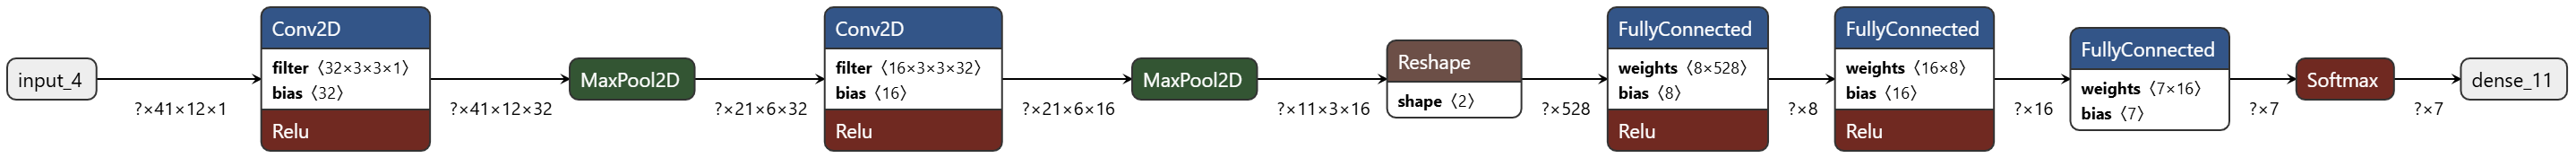
\includegraphics[width=1\linewidth]{Chapters/neuronska_mreza/struktura/model.png} 
    \caption{Neuronska mreža \cite{netron}}
    \label{pic:struktura}
\end{figure}


\section{Treniranje i vrednovanje modela}
\label{sec:training}

Nakon definiranja strukture modela neuronske mreže, na red je došlo treniranje. Podaci 
su u ovom trenutku podijeljeni u skup za treniranje, validacijski te testni skup. Također,
svaki podatak (zvučni zapis) pretvoren je u dvodimenzijsku matricu značajki veličine 41x12.


\begin{lstlisting}[language=C++, caption=Konfiguracija za treniranje, label=code:modelcompile]
model.compile(
    optimizer=tf.keras.optimizers.Adam(),
    loss=tf.keras.losses.SparseCategoricalCrossentropy(),
    metrics=['accuracy'],
)
\end{lstlisting}

U isječku koda \ref{code:modelcompile} prikazana je priprema modela za treniranje.
Za optimizacijski postupak odabran je Adam algoritam (engl. \textit{Adaptive Moment Estimation}).
Adam algoritam je vrsta gradijentnog spusta koja koristi prilagodljivu stopu učenja.
Za funkciju gubitka odabrana je kategorička unakrsna entropija (engl. \textit{Sparse Categorical
Crossentropy}). Ona se koristi za treniranje višeklasnih klasifikacijskih modela, a
matematički je opisana u nastavku \ref{eq:crossentropyloss}.

\begin{equation}
    \label{eq:crossentropyloss}
    L = - \frac{1}{N} \sum_{i=1}^{N} \log p(y_i)
\end{equation}

gdje:
\begin{itemize}
    \item \( L \) je gubitak.
    \item \( N \) je broj uzoraka.
    \item \( y_i \) je oznaka primjera (klasa).
    \item \( p(y_i) \) vjerojatnost predikcije za ispravnu klasu.
\end{itemize}

Nakon prolaska BATCH\_SIZE (u našem slučaju 32) uzoraka kroz mrežu, računa se
gubitak na opisani način te se ažuriraju težine mreže (gradijentnim spustom).
Prolazak svih uzoraka kroz mrežu označava kraj jedne epohe. Treniranje traje 
proizvoljan broj epoha, a u ovom slučaju može se konfigurirati varijablom EPOCHS
(u našem slučaju 50).
Posljednji parametar kojim je konfigurirana mreža je metrika koja se koristi za
vrednovanje modela. U ovom slučaju koristi se točnost (engl. accuracy) koja
predstavlja postotak točno klasificiranih uzoraka u odnosu na ukupan broj uzoraka.

Početak treniranja modela prikazan je u isječku koda \ref{code:training}. Modelu
su predani testni i validacijski skupovi podataka. Uz to, postavljeni su uvjeti ranijeg
zaustavljanja treniranja (engl. \textit{Early Stopping}) jer se može dogoditi da model
konvergira u minimum funkcije gubitka prije isteka predviđenog broja epoha. Nakon
što model prestane smanjivati funkciju gubitka na validacijskom skupu, treniranje
se smatra završenim, a model se sprema u stanje s najmanjim gubitkom (nije nužno 
stanje nakon posljednje odrađene epohe).

\begin{lstlisting}[language=Python, caption=Trening, label=code:training]
history = model.fit(
    train_mfcc_dataset,
    validation_data=validation_mfcc_dataset,
    epochs=EPOCHS ,
    callbacks=tf.keras.callbacks.EarlyStopping(verbose=1, patience=10, restore_best_weights=True),
)
\end{lstlisting}

U nastavku je prikazan proces treniranja. Vidljivo je kako se funkcija
gubitka smanjuje s vremenom, a točnost modela raste. Model je konvergirao nakon 20-ak
epoha te je uzeo stanje s kraja 18. epohe. U postavkama modela namješteno je da se
treniranje ne zaustavi odmah nego da da modelu još određeni broj epoha koji je
u našem slučaju 10 (patience=10).

{
\tiny
%\scriptsize
\begin{verbatim}
Epoch 1/50
662/662 [==============================] - 3s 5ms/step - loss: 1.3427 - accuracy: 0.4707 - val_loss: 0.8837 - val_accuracy: 0.6935
Epoch 2/50
662/662 [==============================] - 3s 5ms/step - loss: 0.9060 - accuracy: 0.6649 - val_loss: 0.6565 - val_accuracy: 0.7714
Epoch 3/50
662/662 [==============================] - 3s 5ms/step - loss: 0.7439 - accuracy: 0.7320 - val_loss: 0.5586 - val_accuracy: 0.8025
Epoch 4/50
662/662 [==============================] - 3s 5ms/step - loss: 0.6457 - accuracy: 0.7659 - val_loss: 0.4887 - val_accuracy: 0.8230
...
Epoch 28/50
662/662 [==============================] - 3s 5ms/step - loss: 0.2817 - accuracy: 0.9040 - val_loss: 0.3869 - val_accuracy: 0.8823
Restoring model weights from the end of the best epoch: 18.
Epoch 28: early stopping
\end{verbatim}
}

Na slici \ref{pic:accuracy} prikazana su dva grafa. Lijevi prikazuje funkciju gubitka
na skupu za treniranje i validacijskom skupu, dok desni prikazuje točnost modela na istim skupovima.
Obje funkcije prikazane su u ovisnosti o broju odrađenih epoha treniranja. Vidljivo je
kako se funkcija gubitka smanjuje s vremenom, a točnost raste. Nakon 20-ak epoha, funkcije
se stabiliziraju. 

\begin{figure}[htb]
    \centering
    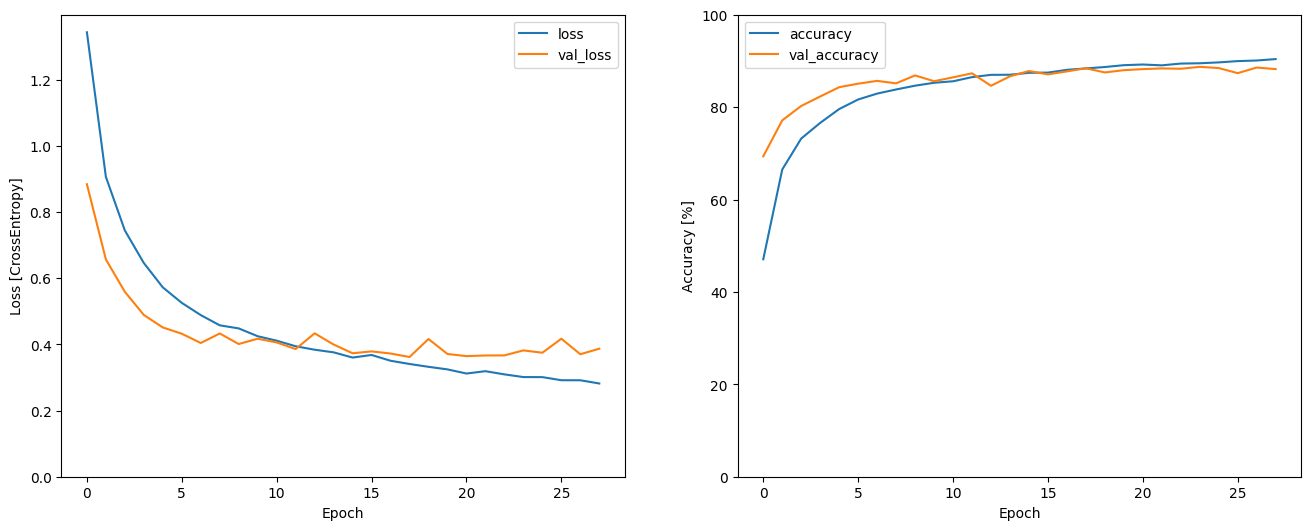
\includegraphics[width=1\linewidth]{Chapters/neuronska_mreza/trening/acc.png} 
    \caption{Gubitak i točnost modela}
    \label{pic:accuracy}
\end{figure}

Konačni iznos funkcije gubitka na testnom skupu iznosi 0.2817, a točnost modela 0.9040, dok
na validacijskom skupu iznosi redom 0.3869 i 0.8823. Međutim, konačna ocjena rezultata
treniranja modela donosi se na temelju testnog skupa. To su podaci koje model nije vidio
niti u jednom trenutku treniranja i predstavljaju podatke kakve će model vidjeti u stvarnom
svijetu. Funkcija gubitka na tom skupu iznosi 0.3480, dok točnost iznosi 0.8814.

Na slici \ref{pic:confmtrx} prikazana je konfuzijska matrica napravljena nad
testnim skupa podataka. Ona prikazuje koliko je puta model pogriješio u klasifikaciji
određene klase. Stupci matrice predstavljaju stvarne klase, a reci predviđene klase
(izlaz treniranog modela). Na dijagonali matrice nalaze se točne klasifikacije, dok
se izvan dijagonale se nalaze pogreške. Vidljivo je kako je model najviše griješio
u klasifikaciji klase "unknown". To je slučaj zbog toga što se u toj klasi nalaze
zvučni zapisi različitih riječi. Drugim riječima, ta klasa je najraznolikija i najteža
za klasificirati te je zbog toga ovakav rezultat očekivan.

\begin{figure}[htb]
    \centering
    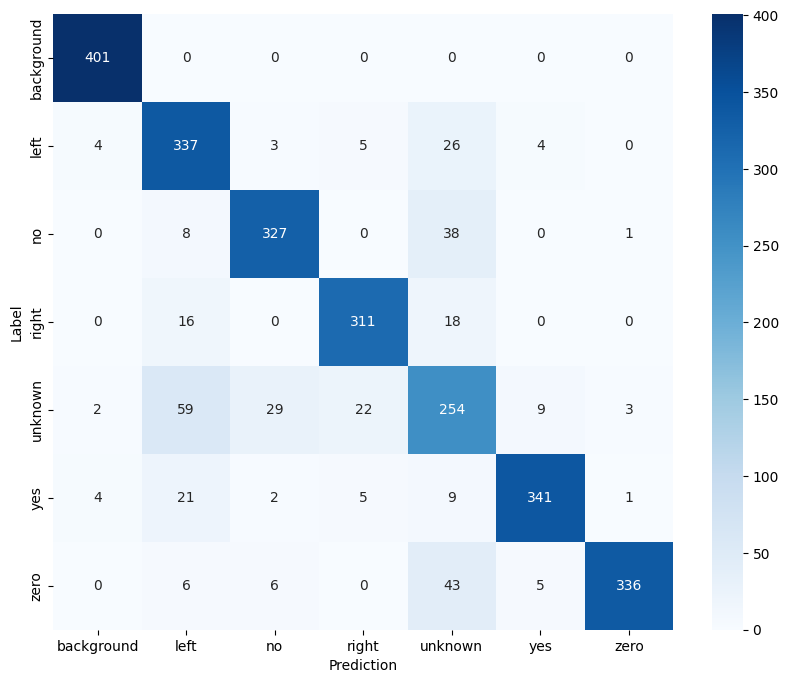
\includegraphics[width=0.7\linewidth]{Chapters/neuronska_mreza/trening/image.png} 
    \caption{Konfuzijska matrica}
    \label{pic:confmtrx}
\end{figure}

\section{Usporedba s drugim modelima na istom skupu podataka}

Usporediti naučeni model s postojećim modelima nije jednostavno zato što
se većina modela temelji na složenijim arhitekturama koje imaju veći broj parametara te
uz svoje rezultate ne prilažu način implementacije na mikrokontroleru. Međutim,
u tablici \ref{tab:models} prikazana je usporedba ovog modela s drugima. Uz naš trenirani model,
ubačen je identičan model treniran na samo dvije glasovne naredbe (ukupno četiri klase).
Iz tablice je vidljivo da naš model zauzima najmanje memorije uz sličnu točnost za 4 klase te
nešto manju za 7 klasa. Točnost bi se jednostavno mogla povećati složenijim potpuno povezanim
slojevima na izlazu trenirane mreže, međutim ovo se čini kao najbolji kompromis između veličine
mreže i njene točnosti.

\begin{table}[htb]
    \centering
    \begin{tabular}{|l|r|r|}
        \hline
        \textbf{Model} & \textbf{Accuracy (\%)} & \textbf{Model Size (KB)} \\ \hline
        Naš CNN (7 klasa) & 88.2 & 15.7 \\ 
        Naš CNN (4 klase) & 93.6 & 15.6 \\ 
        DNN (Deep Neural Network)          \cite{zhang2017hello} & 84.6 & 80 \\
        CNN (Convolutional Neural Network) \cite{zhang2017hello} & 91.6 & 79 \\
        LSTM (Long Short-Term Memory)      \cite{zhang2017hello} & 92.9 & 79.5 \\
        CRNN (Convolutional RNN)           \cite{zhang2017hello} & 94.0 & 79.7 \\
        DS-CNN (Depthwise Separable CNN)   \cite{zhang2017hello} & 94.4 & 38.6  \\
        TripletLoss-res15 \cite{triplet} & 95.2 & 237 \\
        BC-ResNet-8 \cite{res} & 98.7 & 520 \\
        WaveFormer \cite{waveformer} & 98.8 & 130  \\
        \hline
    \end{tabular}
    \caption{Veličine različitih oblika modela i procentualna ušteda}
    \label{tab:models}
\end{table}

\section{Prilagodba za implementaciju na mikrokontroleru}
\label{sec:convert}

Veličina pojedinog sloja treniranog modela neuronske mreže prikazana je u nastavku.
Ukupni broj parametara koje mreža ima iznosi 9439 što u memoriji zauzima malo manje od 
37 KB.

{
\scriptsize
\begin{verbatim}
                      Number of labels: 7            
                      Model: "sequential"
                      _________________________________________________________________
                       Layer (type)                     Output Shape            Param #   
                      =================================================================
                       conv2d (Conv2D)                 (None, 41, 12, 32)        320                                                                       
                       max_pooling2d (MaxPooling2D)    (None, 21, 6, 32)         0                                                                                                                                  
                       conv2d_1 (Conv2D)               (None, 21, 6, 16)         4624                                                                      
                       max_pooling2d_1 (MaxPooling2D)  (None, 11, 3, 16)         0                                                                                                                                    
                       flatten (Flatten)               (None, 528)               0                                                                        
                       dense (Dense)                   (None, 8)                 4232                                                                    
                       dropout (Dropout)               (None, 8)                 0                                                                        
                       dense_1 (Dense)                 (None, 16)                144                                                                      
                       dropout_1 (Dropout)             (None, 16)                0                                                                        
                       dense_2 (Dense)                 (None, 7)                 119                           
                      =================================================================
                      Total params: 9439 (36.87 KB)
                      Trainable params: 9439 (36.87 KB)
                      Non-trainable params: 0 (0.00 Byte)
\end{verbatim}
}

Međutim, spremljeni model u memoriji osim vrijednosti parametara mora imati i informaciju 
o samoj strukturi mreže što znatno povećava sami memorijski otisak. Datoteka s nastavkom
".pb" (engl. \textit{protobuff}) čuva sve informacije potrebne za korištenje treniranog modela,
a konkretni model u tom obliku zauzima nešto više od 173 KB. Korištenje takvog modela
na mikrokontroleru nije prihvatljivo niti zbog veličine niti zbog oblika zapisa. Zbog 
toga je potrebno prilagoditi model. Tensorflow Lite biblioteka omogućava vrlo jednostavnu
promjenu formata spremanja informacije o treniranom modelu. Format s nastavkom ".tflite"
sažima model na nešto više od 41 KB. Međutim, postoji još nešto što je moguće napraviti
kako bi se model sažeo još više te pretvorio u oblik pogodan za korištenje na
mikrokontroleru. Spomenuta metoda sažimanja zove se kvantizacija, a oblik u kojem će model
biti spremljen zove se \textit{flatbuffer}.

Kvantizacija je metoda optimizacije modela kojom se smanjuje broj bitova potrebnih za
spremanje informacije o parametrima modela. 
To je proces mapiranja brojeva s pomičnim zarezom u cijele brojeve.
Ova redukcija preciznosti (s 32 na 8 bitova)
pridonosi smanjenju veličine modela i ubrzanju izvođenja, a neznatno utječe na točnost
modela \cite{quantization}. Ovim zahvatom veličina modela smanjena je na 16 KB. 

\textit{Flatbuffer} je oblik za serijalizaciju podataka razvijen u Googleu. Dizajniran je
za učinkovitu pohranu i pristup podacima \cite{flatbuffers_docs}. 
Pretvorbom treniranog modela u ovakav oblik
dobiveno je polje podataka spremno za korištenje programskim jezikom C.
U isječku programskog koda \ref{code:flatbuffer} prikazan je proces kojim se model pretvara u opisano 
polje.

\begin{lstlisting}[language=C++, caption=Pretvorba u Flatbuffer, label=code:flatbuffer]
# Convert to a C source file
!xxd -i {QUANTIZATION_MODEL} > {MODEL_TFLITE_MICRO}
# Update variable names
REPLACE_TEXT = QUANTIZATION_MODEL.replace('/', '_').replace('.', '_')
!sed -i 's/'{REPLACE_TEXT}'/g_model/g' {MODEL_TFLITE_MICRO}
!cat {MODEL_TFLITE_MICRO}
\end{lstlisting}

Tablica \ref{tab:model_sizes} prikazuje veličine modela u različitim koracima prilagodbe.
Konačni model prihvatljive je veličine za implementaciju na mikrokontrolerskom sustavu, 
a iznosi svega 9\% početne veličine modela.

\begin{table}[htb]
    \centering
    \begin{tabular}{|l|r|r|}
        \hline
        \textbf{Model} & \textbf{Veličina (B)} & \textbf{Udio veličine početnog modela (\%)} \\ \hline
        Početni model & 173241 & 100 \\ \hline
        TF Lite & 41644 & 24.04 \\ \hline
        TF Lite + kvantizacija & 15704 & 9.06 \\ \hline
    \end{tabular}
    \caption{Veličine različitih oblika modela}
    \label{tab:model_sizes}
\end{table}

\chapter{Zaključak}
\label{pog:zakljucak}

Sustav za prepoznavanje govornih naredbi u stvarnom vremenu uspješno je implementiran
na mikrokontrolerskoj platformi ESP32 Lyrat. Nudi jednostavniju modularnu
stukturu od postojećih (\cite{arm_kws}, \cite{tflmicrospeech}) uz sposobnost pouzdanog 
prepoznavanja većeg skupa
naredbi. Implementirani sustav može prepoznati pet
različitih naredbi te aktivirati prikladni posao dodijeljen svakoj naredbi. 
Također, omogućen je odabir 
drugačijeg podskupa govornih naredbi, a uz malo više truda moguće je proširiti skup naredbi
željenim zvučnim zapisima koji će predstavljati naredbu prilagođenu korisniku.
Osim toga, modularna struktura sustava
omogućuje laganu prilagodnu pojedinih dijelova za različite namjene. Na taj način stvorena je
osnova za implementaciju različitih sustava za prepoznavanje drugih vrsta senzorskih podataka
ili čak korištenje drugih vrsta neuronskih mreža. Ono što bi moglo poboljšati sustav
u budučnosti je
nekorištenje brojeva s pomičnim zarezom u generiranju MFC koeficijenata. Na konkretnom
mikontroleru to ne predstavlja prevelik problem zbog jedinice
za operacije s pomičnim zarezom (engl. \textit{Floating Point Unit ili FPU}),
ali na drugim mikrokontrolerima bi takav pristup osjetno ubrzao cijeli proces.





%--- LITERATURA / REFERENCES ---------------------------------------------------

% Literatura se automatski generira iz zadane .bib datoteke / References are automatically generated from the supplied .bib file
% Upiši ime BibTeX datoteke bez .bib nastavka / Enter the name of the BibTeX file without .bib extension
\bibliography{literatura}



%--- SAŽETAK / ABSTRACT --------------------------------------------------------

% Sažetak na hrvatskom
\begin{sazetak}
  Unesite sažetak na hrvatskom.

  
\end{sazetak}

\begin{kljucnerijeci}
  prva ključna riječ; druga ključna riječ; treća ključna riječ
\end{kljucnerijeci}


% Abstract in English
\begin{abstract}
  Enter the abstract in English.
  
 
\end{abstract}

\begin{keywords}
  the first keyword; the second keyword; the third keyword
\end{keywords}


%--- PRIVITCI / APPENDIX -------------------------------------------------------

% Sva poglavlja koja slijede će biti označena slovom i riječi privitak / All following chapters will be denoted with an appendix and a letter
\backmatter

\chapter{Skup podataka za treniranje}


\begin{table}[htb]
    \centering
    \begin{tabular}{|l|r|l|r|}
        \hline
        \textbf{Riječ} & \textbf{Broj zapisa} & \textbf{Riječ} & \textbf{Broja zapisa} \\ \hline
        Backward & 1,664 & Bed & 2,014 \\ \hline
        Bird & 2,064 & Cat & 2,031 \\ \hline
        Dog & 2,128 & Down & 3,917 \\ \hline
        Eight & 3,787 & Five & 4,052 \\ \hline
        Follow & 1,579 & Forward & 1,557 \\ \hline
        Four & 3,728 & Go & 3,880 \\ \hline
        Happy & 2,054 & House & 2,113 \\ \hline
        Learn & 1,575 & Left & 3,801 \\ \hline
        Marvin & 2,100 & Nine & 3,934 \\ \hline
        No & 3,941 & Off & 3,745 \\ \hline
        On & 3,845 & One & 3,890 \\ \hline
        Right & 3,778 & Seven & 3,998 \\ \hline
        Sheila & 2,022 & Six & 3,860 \\ \hline
        Stop & 3,872 & Three & 3,727 \\ \hline
        Tree & 1,759 & Two & 3,880 \\ \hline
        Up & 3,723 & Visual & 1,592 \\ \hline
        Wow & 2,123 & Yes & 4,044 \\ \hline
        Zero & 4,052 & & \\ \hline
        \end{tabular}
    \caption{Broj audio zapisa različitih riječi u skupu \cite{speechcommandsv2}}
    \label{tab:word_frequency}
\end{table}

\end{document}
